This Chapter presents all the experiments performed and the achieved results.
Firstly, some theoretical aspects of each experimental phase are introduced, then all the experiments are clearly illustrated to make them reproducible and the obtained results are explained.

All the CPU experiments have been conducted using an Intel Core i9, with 8 cores and a frequency of 2,3 GHz.
On the other hand, the synthesis experiments utilized an AMD Virtex UltraScale+ (Alveo U280) FPGA\@.

\section{Model analysis and profiling}
\label{sec:model-analysis}%

\begin{table}[b]
\centering
    \begin{tabular}{|p{6em} c c c c|}
    \hline
%    \rowcolor{black!40}
    \textbf{Name} & \textbf{Self CPU \%} & \textbf{Self CPU} & \textbf{CPU total \%} & \textbf{CPU total} \T\B \\
    \hline \hline
    \textbf{aten::mm} & 50,25\% & 1,012$ms$ & 89,72\% & 1,807$ms$ \T\B\\
    \hline
    \textbf{aten::addmm} & 36,30\% & 731,0$\mu s$ & 37,04\% & 746,0$\mu s$ \T\B\\
    \hline
    \textbf{aten::add} & 4,67\% & 94,0$\mu s$ & 4,67\% & 94,0$\mu s$ \T\B\\
    \hline
    %\textbf{aten::\_log\_softmax} & 2,98\% & 60,0us & 2,98\% & 60,0us \T\B\\
    %\hline
    \end{tabular}
    \\[10pt]
    \caption{Excerpt of GCN model inference profiling result}
    \label{tab:gcn_profiling}
\end{table}

As already anticipated in Section~\ref{sec:toolchain-pytorch}, the GCN model, whose class is shown in Listing~\ref{lst:gcn-class}, is implemented in PyTorch, and it is characterized by two convolutional layers, a ReLU and a dropout functions.
The forward function of each layer, shown in Listing~\ref{lst:gcn-layer-forward}, is characterized by two matrix multiplications, and one of the two is a sparse multiplication.

The first step to understanding how to accelerate the PyTorch GCN model used was to analyze and profile it.
Table~\ref{tab:gcn_profiling} shows the results of one result of the profiling done using the PyTorch profiler.

The distinction between \textit{self CPU time} and \textit{total CPU time} lies in the fact that self CPU time does not contain the time spent in child operator calls, whereas total CPU time contains it, considering that operators can invoke other operators.
It is clear that the bottleneck and the most time-consuming operation is the matrix multiplication.
In particular, more than 50\% of the self CPU time is used by matrix multiplication, while, considering the child operator calls, this percentage represents nearly the 90\%.
This result clearly justifies the part of this research dedicated to matrix multiplication acceleration.

\begin{lstlisting}[language=Python,label={lst:gcn-class}, numbers=left, xleftmargin=2em, caption=Class of GCN model]
import torch.nn as nn
import torch.nn.functional as F
from pygcn.layers import GraphConvolution

class GCN(nn.Module):
    def __init__(self, nfeat, nhid, nclass, dropout):
        super(GCN, self).__init__()

        self.gc1 = GraphConvolution(nfeat, nhid)
        self.gc1 = GraphConvolution(nhid, nclass)
        self.dropout = dropout

    def forward(self, x, adj):
        x = F.relu(self.gc1(x, adj))
        x = F.dropout(x, self.dropout,
                      training=self.training)
        x = self.gc2(x, adj)
        return F.log_softmax(x, dim=1)
\end{lstlisting}


\begin{lstlisting}[language=Python,label={lst:gcn-layer-forward}, numbers=left, xleftmargin=2em, caption=Forward function of GCN layer]
    def forward(self, input, adj):
        support = torch.mm(input, self.weight)
        output = torch.spmm(adj, support)
        if self.bias is not None:
            return output + self.bias
        else:
            return output
\end{lstlisting}

\section{Matrix multiplication acceleration}
\label{sec:matmul-acceleration}%

Matrix multiplication is a well-known algorithm.
It consists of multiplying two compatible matrices to obtain the result matrix.
A lot of work has been done to try to improve its performance on different architectures~\cite{DBLP:journals/corr/abs-2003-00532, opt_cuda_matmul}.

The naive implementation of the row-by-column multiplication, whose pseudocode is shown below, is characterized by three nested loops.
The multiplication is possible only in the case the number of column of the first matrix is equal to the number of row of the second one.

\begin{algorithm}[H]
    \label{alg:matmul_pseudo}
    \caption{Naive matrix multiplication algorithm}
    \label{alg:var}
    \label{protocol1}
    \begin{algorithmic}[1]
    \STATE \textbf{Data:} $A[R][P], B[M][N]$
    \STATE \textbf{Result:} $C[R][N]$
    \IF{$P == M$}
    \FOR{$m=0; m<R, m++$}
    \FOR{$r=0; r<N, r++$}
    \STATE $C[m][r] = 0$
    \FOR{$k=0; k<M, k++$}
    \STATE $C[m][r] += A[m][k] * B[k][r]$
    \ENDFOR
    \ENDFOR
    \ENDFOR
    \ENDIF
    \end{algorithmic}
\end{algorithm}

\begin{figure}[t]
    \centering
    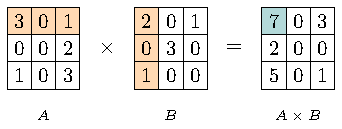
\includegraphics[height=0.24\textwidth]{Images/row-by-col-mult-example}
    \caption{Row-by-column matrix multiplication example}
    \label{fig:row-by-col-mul-example}
\end{figure}

Figure~\ref{fig:row-by-col-mul-example} highlight how an element of the output matrix is computed, using a row of the first matrix and a column of the second one.
The number of operations needed to compute a new matrix is an important parameter to try to accelerate such operation.
A calculus of this number preceded each experiments, to compute an approximation of the number of cycles needed by the accelerator.
In a general matrix multiplication, shown in Equation~\ref{eq:matmul}, each element of the new matrix can be computed accordingly to Equation~\ref{eq:matmul-element}.

\begin{equation}
        \label{eq:matmul}
    \begin{bmatrix}
     a_{11} & a_{12} & \cdots & a_{1n}\\
     a_{21} & a_{22} & \cdots & a_{2n}\\
     \vdots & \vdots & \ddots & \vdots\\
     a_{m1} & a_{m2} & \cdots & a_{mn}
 \end{bmatrix}
 \times
 \begin{bmatrix}
     b_{11} & b_{12} & \cdots & b_{1p}\\
     b_{21} & b_{22} & \cdots & b_{2p}\\
     \vdots & \vdots & \ddots & \vdots\\
     b_{n1} & b_{n2} & \cdots & b_{np}
 \end{bmatrix}
  =
 \begin{bmatrix}
     c_{11} & c_{12} & \cdots & c_{1p}\\
     c_{21} & c_{22} & \cdots & c_{2p}\\
     \vdots & \vdots & \ddots & \vdots\\
     c_{m1} & c_{m2} & \cdots & c_{mp}
 \end{bmatrix}
\end{equation}

\begin{equation}
    \label{eq:matmul-element}
    c_{ij}= a_{i1} b_{1j} + a_{i2} b_{2j} +\cdots+ a_{in} b_{nj} = \sum_{k=1}^n a_{ik}b_{kj}
\end{equation}

Then, the number of cycles needed can be calculated using Equation~\ref{eq:number-cycles}.
The notation used refers to Equation~\ref{eq:matmul}, but it can be referred to Algorithm~\ref{alg:var} by considering $n = M \land m=R \land p=N$
The first part of the Equation computes the total number of iterations, while the second half computes the number of cycles needed to perform multiplications and additions, and to load and store data.
The number of cycles needed to load and store data are computed by adding one cycle for each $ch$ operands read, and one cycle for each $ch$ operand written, with $ch$ equal to the number of memory channels.
From Listing~\ref{lst:affine-mul}, it can be seen that there are three load and one store, for a total of four memory operations.

\begin{equation}
    \label{eq:number-cycles}
    cycles = \left(  n \cdot m \cdot p \right) \cdot \left(  cycles_{mul} + cycles_{add} + \frac{4}{ch} \right)
\end{equation}

Let us consider two matrices, the first of size $15\times15$ and the second of size $15\times16$.
The FPGA model used for the experimental phase uses three cycles for addition and two cycles for multiplication.
By applying the Equation~\ref{eq:number-cycles}, the expected number of cycles for computing such matrix multiplication, using two memory channels is 25,200.

\subsection{PyTorch matrix multiplication benchmark}
\label{subsec:pytorch-matmul-bench}%

PyTorch provides different matrix representations and different matrix multiplication functions.
The one considered in this Subsection are \textit{torch.mm} and \textit{torch.spmm}.
The former function multiplies two dense matrices, but it also supports COO representation.
The latter, instead, is typically used for sparse matrix multiplications, in which one of the two matrices, or both, are saved using sparse representations.

Figure~\ref{fig:torch-mm_benchmark} represents a benchmark for the dense matrix multiplication between a first matrix of size $15 \times 15$ and a second matrix of size $15 \times 16$, both composed by float32 elements.
In particular, the plot shows five measurements computed as the average of five different executions' number.
Additionally, this average has been computed five times, and the red bar shows the range between the minimum and the maximum execution time of these repetitions.

As expected, given the high amount of executions, the five average execution times are similar between them, and the red range bar decreases as the number of executions increases.
In conclusion, the time needed by a dense matrix multiplication between two matrices of the given size can be considered equal to 1.608$\mu s$.
The Python timing of the accelerated functions for each experiment has been computed using an average of ten millions executions.

Since the GCN model uses both dense and sparse matrix multiplication functions, Table~\ref{tab:torch-matmul-comparison} shows the times needed by both functions according to different representations of the two input matrices A and B\@.
All the times have been computed as the average of ten millions executions, the two matrices are both of size $20 \times 20$ and randomly generated; they are both composed by float32 elements and COO matrices have a sparsity of 90\%.

\begin{table}[t]
\centering
    \begin{tabular}{|p{6em} c c c |}
    \hline
    \textbf{Function} & \textbf{Dense$\times$Dense} & \textbf{COO$\times$Dense} & \textbf{COO$\times$COO} \T\B \\
    \hline \hline
    \textbf{torch.mm} & 1.840$\mu s$  & 3.299$\mu s$ & 16.855$\mu s$ \T\B\\
    \hline
    \textbf{torch.spmm} & 1.875$\mu s$  & 3.234$\mu s$ & 15.215$\mu s$ \T\B\\
    \hline
    \end{tabular}
    \\[10pt]
    \caption{Comparison between dense and sparse PyTorch matmul functions}
    \label{tab:torch-matmul-comparison}
\end{table}

\begin{figure}[t]
    \centering
    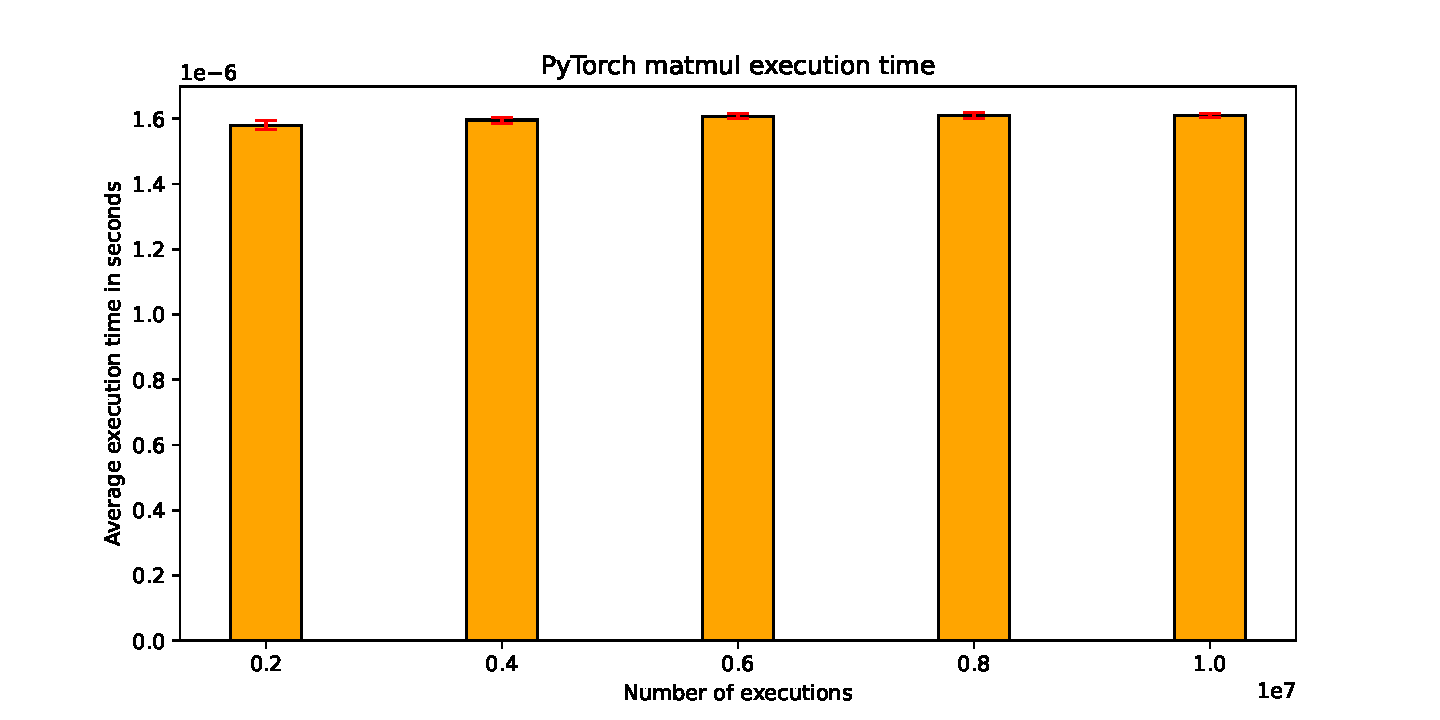
\includegraphics[height=0.4\textwidth]{Images/torch-mm_benchmark}
    \caption{Benchmark of \textit{torch.mm} PyTorch function}
    \label{fig:torch-mm_benchmark}
\end{figure}

It is clear that sparse matrix multiplication, both with dense and sparse matrix representations, does not increase performance on CPU architecture.
The disadvantage of using sparse matrix multiplication on CPU becomes more and more evident as the size of the input matrices increases.

\subsection{Optimization comparison}
\label{subsec:optimization-comparison}%

Before applying any SODA-OPT or PandA-Bambu optimization, it is necessary to understand the difference between PyTorch matrix multiplication operation and the baseline accelerator.
Table~\ref{tab:pytorch-accelerator-comparison} and Figure~\ref{fig:pytorch-accelerator-comparison} show the result of this analysis.
The PyTorch times have been recorded by averaging five measurements each of ten millions executions.
The baseline accelerator is much faster than PyTorch when matrices are relatively small.
The difference of performance decreases as the size of the input matrices increase until reaching a point in which the accelerator becomes slower than PyTorch solution.

\begin{table}[t]
\centering
    \begin{tabular}{|p{9em} c c c c  |}
    \hline
    \textbf{Input sizes} & \textbf{Torch.mm (s)} & \textbf{Runtime (s)} & \textbf{Cycles} & \textbf{SpeedUp} \T\B \\
    \hline \hline
    \textbf{15$\times$15, 15$\times$16} & 1.608E-06  & 96.492E-09 & 25,697 & 16.664 \T\B\\
    \hline
    \textbf{30$\times$30, 30$\times$16} & 1.733E-06  & 351.182E-09 & 101,792 & 4.934 \T\B\\
    \hline
    \textbf{60$\times$60, 60$\times$16} & 2.480E-06  & 1.466E-06 & 405,182 & 1.691 \T\B\\
    \hline
    \textbf{90$\times$90, 90$\times$16} & 4.554E-06  & 3.150E-06 & 910,172 & 1.445 \T\B\\
    \hline
    \textbf{120$\times$120, 120$\times$16} & 4.792E-06  & 00.000E-06 & 00,000 & 16.664 \T\B\\
    \hline
    \textbf{150$\times$150, 150$\times$16} & 5.161E-06  & 9.074E-06 & 2,524,952 & 0.568 \T\B\\
    \hline
    \end{tabular}
    \\[10pt]
    \caption{Comparison between dense and sparse PyTorch matmul functions}
    \label{tab:pytorch-accelerator-comparison}
\end{table}

\begin{figure}[t]
    \centering
    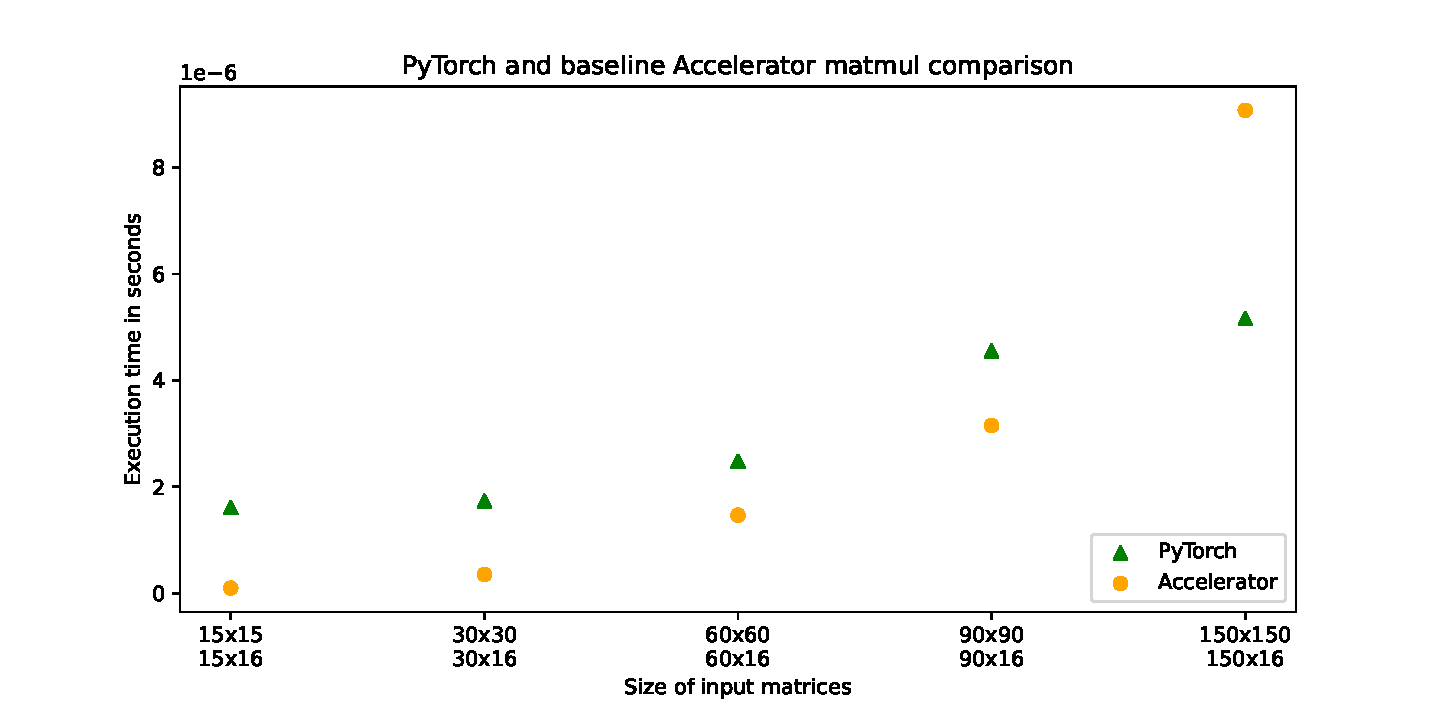
\includegraphics[height=0.4\textwidth]{Images/matmul_comparison}
    \caption{Performance comparison between PyTorch matmul function and accelerator}
    \label{fig:pytorch-accelerator-comparison}
\end{figure}

\begin{lstlisting}[label={lst:affine-mul-unroll3}, caption=Unrolled matrix multiplication in affine dialect with unrolling factor 3]
affine.for %arg3 = 0 to 15 {
  affine.for %arg4 = 0 to 16 {
    affine.for %arg5 = 0 to 15 step 3 {
      %0 = affine.load %arg0[%arg3, %arg5] : memref<15x15xf32>
      %1 = affine.load %arg1[%arg5, %arg4] : memref<15x16xf32>
      %2 = affine.load %arg2[%arg3, %arg4] : memref<15x16xf32>
      %3 = arith.mulf %0, %1 : f32
      %4 = arith.addf %2, %3 : f32
      affine.store %4, %arg2[%arg3, %arg4] : memref<15x16xf32>
      %5 = affine.apply affine_map<(d0) -> (d0 + 1)>(%arg5)
      %6 = affine.load %arg0[%arg3, %5] : memref<15x15xf32>
      %7 = affine.load %arg1[%5, %arg4] : memref<15x16xf32>
      %8 = affine.load %arg2[%arg3, %arg4] : memref<15x16xf32>
      %9 = arith.mulf %6, %7 : f32
      %10 = arith.addf %8, %9 : f32
      affine.store %10, %arg2[%arg3, %arg4] : memref<15x16xf32>
      %11 = affine.apply affine_map<(d0) -> (d0 + 2)>(%arg5)
      %12 = affine.load %arg0[%arg3, %11] : memref<15x15xf32>
      %13 = affine.load %arg1[%11, %arg4] : memref<15x16xf32>
      %14 = affine.load %arg2[%arg3, %arg4] : memref<15x16xf32>
      %15 = arith.mulf %12, %13 : f32
      %16 = arith.addf %14, %15 : f32
      affine.store %16, %arg2[%arg3, %arg4] : memref<15x16xf32>
    }
  }
}
\end{lstlisting}

This behaviour can be attributed to the fact that PyTorch times have been recorded using all the eight available threads on the machine.
So, the \lstinline{torch.mm} function exploits more parallelism with respect to the accelerator.
For this reason, the optimizations discussed in Section~\ref{subsec:toolchain-soda_opt} and in Section~\ref{subsec:toolchain-panda_bambu} and evaluated in the following makes the accelerator able to exploit more parallelism.

To verify the effectiveness of the proposed optimizations, different comparative analysis have been performed.
SODA-OPT offers the possibility to make different types of unrolling, among which the full unroll which completely unroll the innermost loop, and the partial unroll up to an arbitrary factor.
Listing~\ref{lst:affine-mul-unroll3} shows the effect of a partial unrolling, with unrolling factor equal to 3, to the matrix multiplication introduced in Listing~\ref{lst:affine-mul}.

PandA-Bambu introduces several optimization options, one of which involves expanding the number of memory channels in use.
By default, the system employs two channels and utilizes \lstinline{ALL_BRAM} as the memory allocation policy, directing all objects to be stored in BRAMs.
However, there's an alternative approach explored in this thesis, which entails employing a greater number of memory channels while utilizing external memory, approach that appears to be in line with the coalescent accesses performed on CUDA.
To achieve this, the \lstinline{NO_BRAM} memory allocation policy must be selected, leading to all objects being stored in external memory.

This choice offers both advantages and disadvantages, resulting in a trade-off.
Loop unrolling enhances parallelization, thereby reducing computational time.
However, especially when utilizing more than two memory channels, it increases the number of parallel processing elements, leading to a larger area footprint.
Additionally, external memory allows for up to 32 memory channels, enabling the simultaneous loading of 32 variables.
Nonetheless, accessing data from external memory requires more load cycles compared to accessing internal memory.

The conducted analyses aim to highlight the differences among these various configurations, identifying the optimal balance between reducing cycles and containing area utilization.

\begin{figure}[t]
    \centering
    \subfloat[Input matrices $15\times15$, $15\times16$\label{fig:matmul-optimization-comparison15}]{
        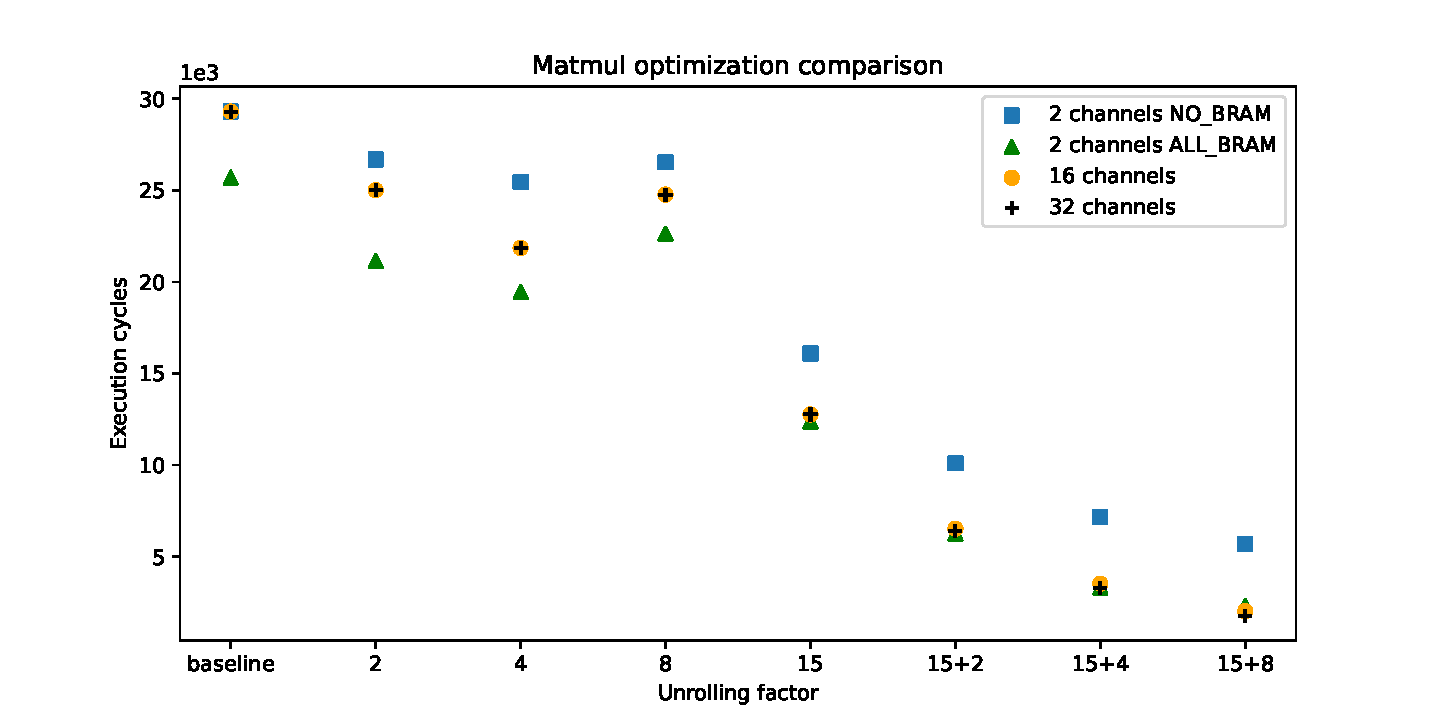
\includegraphics[height=0.4\textwidth]{Images/matmul_comparison15}
    }
    %\quad
    \hspace{0.15\textwidth}
    \subfloat[Input matrices $30\times30$, $30\times16$\label{fig:matmul-optimization-comparison30}]{
        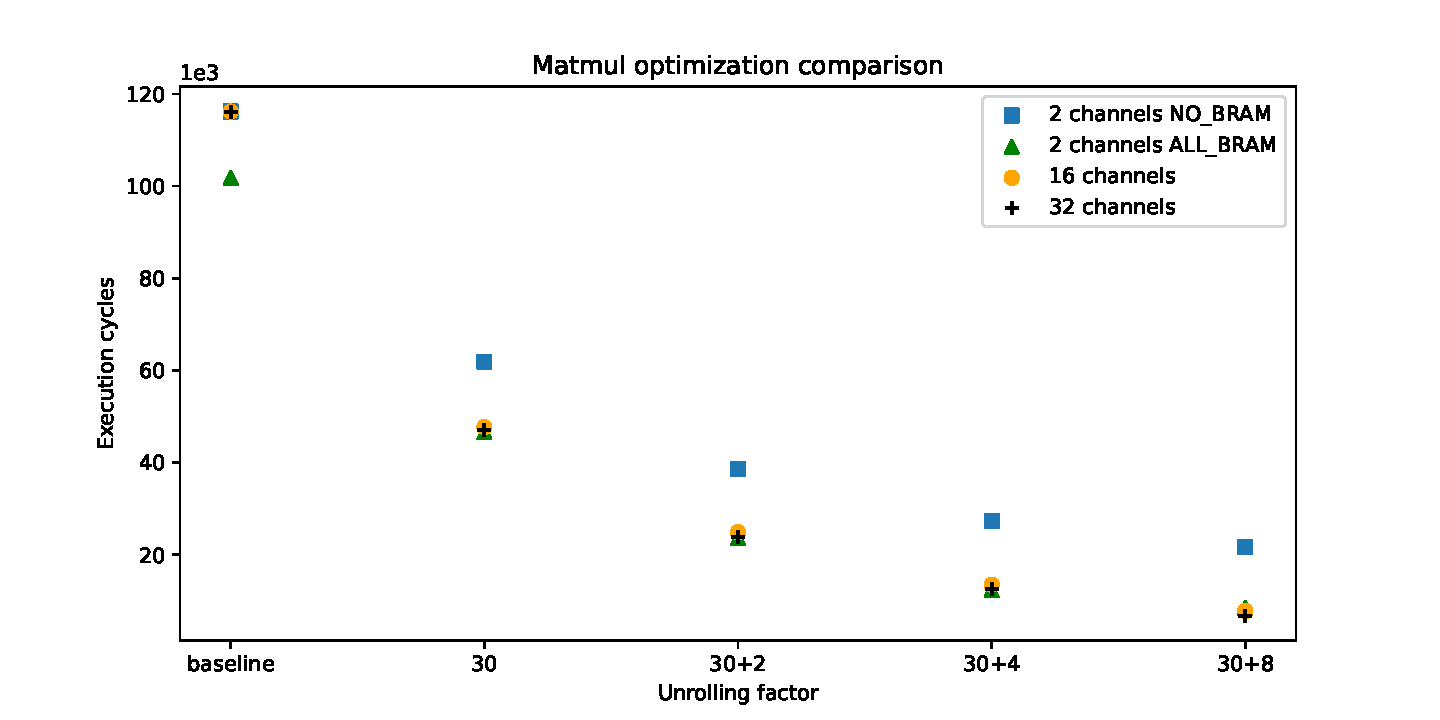
\includegraphics[height=0.4\textwidth]{Images/matmul_comparison30}
    }
    \caption{Matrix multiplication optimization comparison}
    \label{fig:matmul-optimization-comparison}
\end{figure}

Figure~\ref{fig:matmul-optimization-comparison} show two matrix multiplication analyzes performed using different sizes of the input matrices.
Figure~\ref{fig:matmul-optimization-comparison15} show results of a multiplication between two matrices of size $15\times15$ and $15\times16$, while Figure~\ref{fig:matmul-optimization-comparison30} shows results of a multiplication between two matrices of size $30\times30$ and $30\times15$.
In both figures, on the abscissa there is the unrolling factor used and on the ordinate the resulting number of cycles.
The baseline computation does not use unrolling, instead when there are two factors it means that the first one can be considered as a full unroll of the innermost cycle, while the second one is the unrolling factor applied to the original second innermost cycle.

In both cases, when the parallelization is not high, thus the unrolling factor is small, using two channels is the best option since a minor number of cycles is required to perform the computation.
Using 16 channels seems to be similar to use 32 channels, but when parallelization is high the former option uses fewer cycles.

The most important result is given by the unrolling factor in which the number of cycles needed by the accelerator using 32 memory channels is fewer than the number of cycles needed by the accelerator using 2 memory channels.
In the first case, in Figure~\ref{fig:matmul-optimization-comparison15}, this objective is achieved with two unrolling factors of 15 and 8, while in the second case is achieved with unrolling factors of 30 and 8.

These two results, since the unrolling factors are not equals, could appear unrelated.
Using 15 and 8 as unrolling factors means having $15 \cdot 8 = 120$ parallel loop iterations.
Instead, using 30 and 8 as unrolling factors means having $30 \cdot 8 = 240$ parallel loop iterations.

The total amount of possible parallel loop iterations in a matrix multiplication between two matrices of sizes $15\times15$ and $15\times16$ is equal to $15 \cdot 16 \cdot 15 = 3,600$.
Meanwhile, the total amount of possible parallel loop iterations in a matrix multiplication between two matrices of sizes $30\times30$ and $30\times16$ is $30 \cdot 16 \cdot 30 = 14,400$.

Even if the two number of parallel loop iterations representing the changing point of the trade-off, 120 and 240, are different, they are related by the following Equation:
\begin{equation}
    \label{eq:factor-relation}
        2 \cdot \sqrt {M \cdot N \cdot R} = i \cdot j \cdot k
\end{equation}

where $M$, $N$ and $R$ are the sizes of the three nested loops, as defined in Algorithm~\ref{alg:var}, and $i$, $j$ and $k$ are their respective loop unrolling factors, following the rule $j \neq 1 \iff i=M \land k \neq 1 \iff j=N$.

Equation~\ref{eq:factor-relation} should not be taken as an infallible rule, it is the outcome of this experimental phase and should be used as a discriminant to decide when to use thirty-two memory channels instead of two.
In conclusion, the generalized rule, outcome of this comparative analysis is that using thirty-two channels is preferred and convenient when the number of parallel loop iterations is greater than the one computed using Equation~\ref{eq:factor-relation}.

\subsection{GCN accelerator evaluation}
\label{subsec:gcn_accelerator_evaluation}%

In this Subsection, the ultimate evaluation of the optimizations examined and suggested in Subsection~\ref{subsec:optimization-comparison} is presented, aimed at understanding their influence on GCN inference time.

As previously mentioned in the previous Subsection, Table~\ref{tab:pytorch-accelerator-comparison} shows the cycle counts required by the accelerator for each experiment.
These counts align perfectly with the anticipated expectations outlined in Equation~\ref{eq:number-cycles}.
Specifically, dividing the cycle count of the first experiment of the table and the final one by the total count of loop iterations effectively confirms a consistent result of approximately 7 in both instances, confirming that the number of cycles per each loop iteration stayed constant.

\begin{table}[t]
\centering
    \resizebox{\textwidth}{!}{
    \begin{tabular}{|p{4em} c c c c c c|}
    \hline
    \thead{Dataset} & \thead{PyTorch (s)} & \thead{Optimizations} & \thead{Runtime (s)} & \thead{Cycles} & \thead{Area} & \thead{SpeedUp} \T\B \\
    \hline \hline
    \makecell{Cora15} & 59.25E-06 & \makecell{32 channels \\ Unrolling} & 0E-09 & 0 & 0 & 0 \T\B\\
    \hline
    \makecell{Cora30} & 66.42E-06 & \makecell{32 channels \\ Unrolling} & 0E-09 & 0 & 0 & 0 \T\B\\
    \hline
    \makecell{Cora60} & 69.75E-06 & \makecell{32 channels \\ Unrolling} & 0E-09 & 0 & 0 & 0 \T\B\\
    \hline
    \makecell{Cora90} & 88.88E-06 & \makecell{32 channels \\ Unrolling} & 0E-09 & 0 & 0 & 0 \T\B\\
    \hline
    \makecell{Cora120} & 98.32E-06 & \makecell{32 channels \\ Unrolling} & 0E-09 & 0 & 0 & 0 \T\B\\
    \hline
    \makecell{Cora150} & 115.03E-06 & \makecell{32 channels \\ Unrolling} & 0E-09 & 0 & 0 & 0 \T\B\\
    \hline
    \end{tabular}}
    \\[10pt]
    \caption{GCN inference time comparison}
    \label{tab:GCN-inference-pytorch-accelerator-comparison}
\end{table}

\begin{figure}[t!]
    \centering
    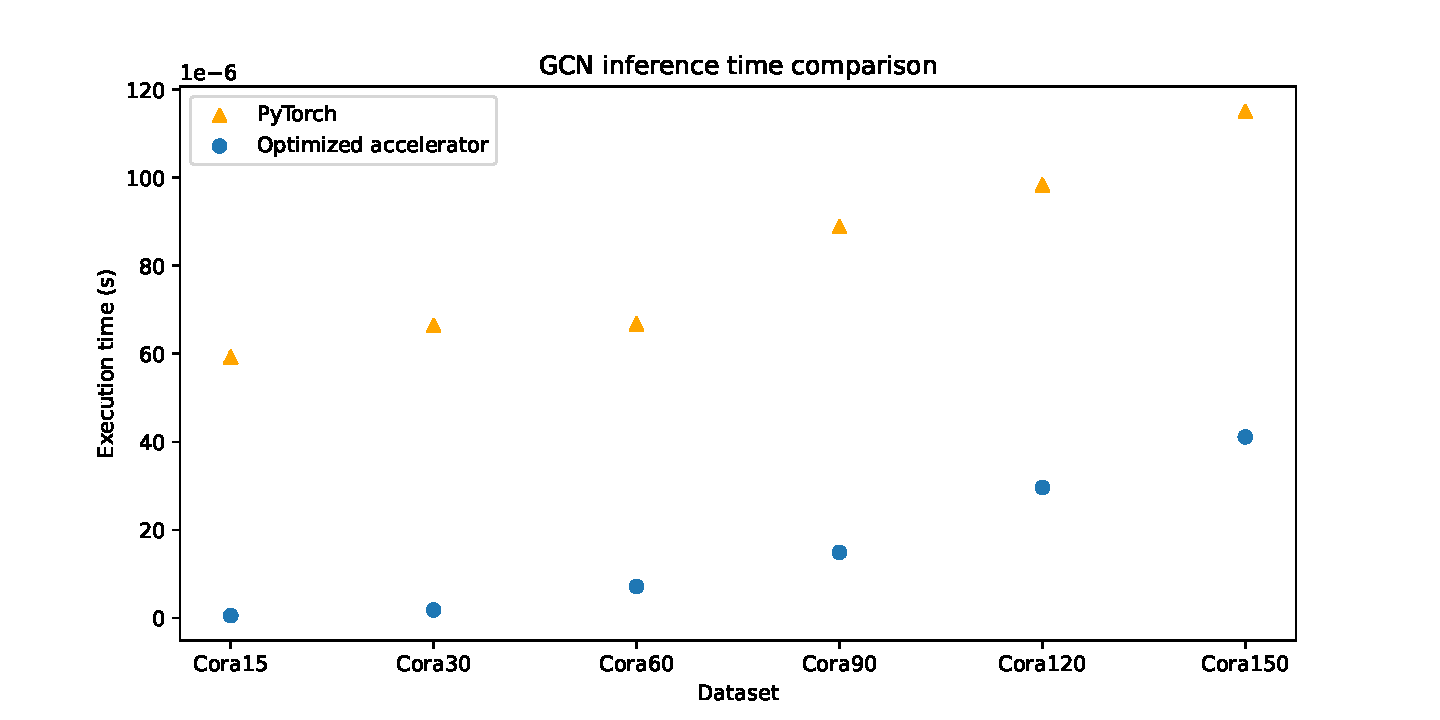
\includegraphics[height=0.4\textwidth]{Images/gcn_forward_comparison}
    \caption{GCN inference time comparison}
    \label{fig:gcn-inference-comparison}
\end{figure}

However, this behavior limits the utilization of the possibilities presented by FPGA technology, which encompass substantial parallelization potential and concurrent memory accesses.

Figure~\ref{fig:gcn-inference-comparison} and Table~\ref{tab:GCN-inference-pytorch-accelerator-comparison}, show the result of a comparative analysis between the PyTorch CPU time and the FPGA accelerator time to perform GCN inference.
The PyTorch times have been acquired averaging one million of execution time measurements using the PyTorch built-in benchmark API\@.

The results of this final evaluation are incredibly encouraging.
The speedup of the accelerator is not being affected by the size of the input matrices and its computation time is significantly lower with respect to the one measured on CPU with PyTorch.

The area of the accelerator, instead, is obviously affected by the sizes of the input matrices.
This because more the matrices are big, more the parallel loop iterations will be and thus the parallel processing elements.

However, the possibilities offered by the proposed toolchain are various.
It is possible to use less memory channels with a lower loop unrolling factor to still have a big positive impact on performance, but containing the accelerator area requirements.

